% interactcadsample.tex
% v1.03 - April 2017

\documentclass[]{interact}

\usepackage{epstopdf}% To incorporate .eps illustrations using PDFLaTeX, etc.
\usepackage{subfigure}% Support for small, `sub' figures and tables
%\usepackage[nolists,tablesfirst]{endfloat}% To `separate' figures and tables from text if required

\usepackage{natbib}% Citation support using natbib.sty
\bibpunct[, ]{(}{)}{;}{a}{}{,}% Citation support using natbib.sty
\renewcommand\bibfont{\fontsize{10}{12}\selectfont}% Bibliography support using natbib.sty

\theoremstyle{plain}% Theorem-like structures provided by amsthm.sty
\newtheorem{theorem}{Theorem}[section]
\newtheorem{lemma}[theorem]{Lemma}
\newtheorem{corollary}[theorem]{Corollary}
\newtheorem{proposition}[theorem]{Proposition}

\theoremstyle{definition}
\newtheorem{definition}[theorem]{Definition}
\newtheorem{example}[theorem]{Example}

\theoremstyle{remark}
\newtheorem{remark}{Remark}
\newtheorem{notation}{Notation}


% tightlist command for lists without linebreak
\providecommand{\tightlist}{%
  \setlength{\itemsep}{0pt}\setlength{\parskip}{0pt}}



\usepackage{lscape}
\usepackage{hyperref}
\usepackage[utf8]{inputenc}
\def\tightlist{}
\usepackage{xcolor}
\definecolor{orange-red}{rgb}{1.0, 0.27, 0.0}
\newcommand{\svp}[1]{{\textcolor{orange-red}{#1}}}
\newcommand*{\Perm}[2]{{}^{#1}\!P_{#2}}%

\usepackage{booktabs}
\usepackage{longtable}
\usepackage{array}
\usepackage{multirow}
\usepackage{wrapfig}
\usepackage{float}
\usepackage{colortbl}
\usepackage{pdflscape}
\usepackage{tabu}
\usepackage{threeparttable}
\usepackage{threeparttablex}
\usepackage[normalem]{ulem}
\usepackage{makecell}
\usepackage{xcolor}

\begin{document}


\articletype{ARTICLE TEMPLATE}

\title{Why is it that statistical tests for residuals are not widely
used? An explanation using visual inference.}


\author{\name{Weihao Li$^{a}$, Dianne Cook$^{a}$, Emi
Tanaka$^{a}$, Susan VanderPlas$^{b}$}
\affil{$^{a}$Department of Econometrics and Business Statistics, Monash
University, Clayton, VIC, Australia; $^{b}$Department of Statistics,
University of Nebraska, Lincoln, Nebraska, USA}
}

\thanks{CONTACT Weihao
Li. Email: \href{mailto:weihao.li@monash.edu}{\nolinkurl{weihao.li@monash.edu}}, Dianne
Cook. Email: \href{mailto:dicook@monash.edu}{\nolinkurl{dicook@monash.edu}}, Emi
Tanaka. Email: \href{mailto:emi.tanaka@monash.edu}{\nolinkurl{emi.tanaka@monash.edu}}, Susan
VanderPlas. Email: \href{mailto:susan.vanderplas@unl.edu}{\nolinkurl{susan.vanderplas@unl.edu}}}

\maketitle

\begin{abstract}
Abstract to fill.
\end{abstract}

\begin{keywords}
data visualization; visual inference; hypothesis testing; residual
plots;
\end{keywords}

\hypertarget{introduction}{%
\section{Introduction}\label{introduction}}

\begin{quote}
\emph{``Since all models are wrong the scientist must be alert to what
is importantly wrong.''} \citep{box1976science}
\end{quote}

Diagnosing a model is the key to determining whether there is anything
importantly wrong. In linear regression analysis, residuals are
typically examined for model diagnostics. Residuals summarise what is
not captured by the model, and thus provide the capacity to identify
what might be wrong.

One can access residuals in multiple ways. Residuals might be plotted,
as a histogram or quantile-quantile plot to examine the distribution.
Using the classical normal linear regression model as an example, if the
distribution is symmetric and unimodal, it is well-behaved. But if the
distribution is skewed, bimodal, multimodal, or contains outliers, there
is cause for concern. One could also inspect the distribution by
conducting a goodness of fit test, such as the Shapiro-Wilk Normality
test \citep{shapiro1965analysis}.

More typically, residuals will be plotted, as a scatter plot against the
predicted values and each of the explanatory variables to scrutinize
their relationships. If there are any visually discoverable patterns,
the model is potentially misspecified. In general, one looks for
noticeable departures from the model like non-linear dependency or
heteroskedasticity. However, correctly judging a residual plot where no
pattern exists is a painstakingly difficult task for humans (?citation).
It is especially common, particularly among new data analysts, to report
patterns when an experienced one might quickly conclude that there are
none. It is also possible to conduct hypothesis tests for non-linear
dependence \citep{ramsey_tests_1969}, and use a Breusch-Pagan test
\citep{breusch_simple_1979} for heteroskedasticity.

Abundance of literature describe appropriate diagnostic methods for
linear regression: \citet{draper1998applied},
\citet{montgomery1982introduction}, \citet{belsley_regression_1980},
\citet{cook_applied_1999} and \citet{cook1982residuals}. The diligent
reader of these sage writings will also notice sentences that express
sentiments like \emph{based on their experience, statistical tests are
not widely used in regression diagnostics since the same or even larger
amount of information can be provided by diagnostic plots than the
corresponding tests in most empirical studies.} A common guidance by
experts is that optimal method for diagnosing model fits is by plotting
the data.

The persistence of this advice to check the plots is curious, and
investigating why this might be common advice is the subject of this
paper. The paper is structured as follows. The next background section
describes the types of departures that one expects to detect, and
outlines a formal statistical process for reading residual plots, called
visual inference. Section \ref{experimental-design} details the
experimental design to compare the decision made by formal hypothesis
testing, and how humans would read diagnostic plots. The results are
reported in Section \ref{results}. We finish with a discussion on future
work, in particular how the responsibility for residual plot reading
might be relieved.

\hypertarget{background}{%
\section{Background}\label{background}}

\hypertarget{departures-from-good-residual-plots}{%
\subsection{Departures from good residual
plots}\label{departures-from-good-residual-plots}}

\begin{figure}

{\centering 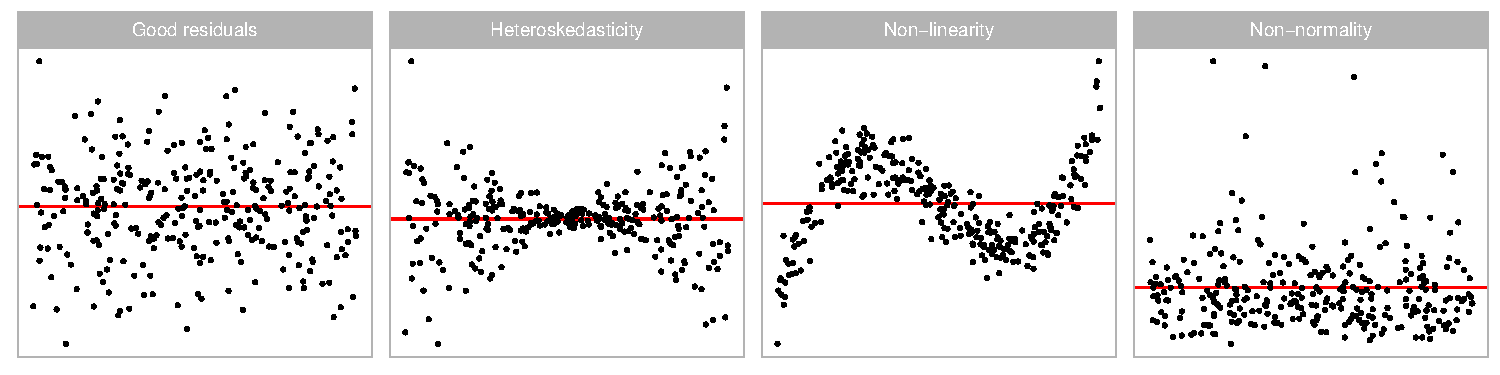
\includegraphics[width=1\linewidth]{paper_comparison_files/figure-latex/residual-plot-common-departures-1} 

}

\caption{Example fitted vs residual plots: (A) classically good looking residuals, (B) non-linear pattern indicates that the model has not captured a non-linear association, (C) heteroskedasticity indicating that variance around the fitted model is not uniform, and (D) non-normality where the residual distribution is not symmetric around 0. The latter pattern might best be assessed using a univariate plot of the residuals, but patterns B and C need to be assessed using a residual vs fitted plot.}\label{fig:residual-plot-common-departures}
\end{figure}

Graphical summaries in which residuals are plotted against fitted values
or other functions of the regressors that are approximately orthogonal
to residuals are referred to as standard residual plots in
\citet{cook1982residuals}. As shown in Figure
\ref{fig:residual-plot-common-departures}, the plot A is an ideal
residual plot with residuals evenly distributed at both sides of the
horizontal zero line, with no noticeable patterns.

There are various types of departures from an ideal residual plot.
Non-linearity, heterskedasticity and non-normality are perhaps the three
mostly checked departures.

Non-linearity is a type of model misspecification caused by failing to
include higher order terms of the regressors in the regression equation.
Any non-linear functional form of residuals on fitted values presented
in the residual plot could be considered as an indicative of
non-linearity. An example residual plot containing visual pattern of
non-linearity is given at plot B of Figure
\ref{fig:residual-plot-common-departures}. One can clearly observe the
``S-shape'' from the residual plot as the cubic term is not captured by
the misspecified model.

Heteroskedasticity refers to the presence of nonconstant error variance
in a regression model. It is mostly due to the strict but false
assumptions on the variance-covariance matrix of the error term. The
usual pattern of heteroskedasticity on a residual plot is the
inconsistent spread of the residuals across the horizontal axis.
Visually, it sometimes results in the so-called ``butterfly'' shape as
shown in the plot C of Figure \ref{fig:residual-plot-common-departures},
or the ``left-triangle'' and ``right-triangle'' shape where the smallest
variance occurs at one side of the horizontal axis.

Compared to non-linearity and heteroskedasticity, non-normality is
usually harder to detect from a residual plot since a scatter plot do
not readily reveal the marginal distribution. A favourable graphical
summary for this task is the quantile-quantile plot. Hence,
non-normality will not be the focus of this paper as we mainly discuss
residual plots. For a consistent comparison, the residual plot of this
departure is still presented in plot D of Figure
\ref{fig:residual-plot-common-departures}. Besides, it is important to
note that not all regression models assume normality for the error term,
but a certain amount do including the classical normal linear regression
model. In the case that the normality assumption is violated, it is
expected to observe data points do not center around the horizontal axis
and there is an uneven distribution of the number points at both below
and above the horizontal axis. For example, given a skewed error
distribution, there will be fewer data points and more outliers on one
side of the horizontal axis as shown in plot D of Figure
\ref{fig:residual-plot-common-departures}.

\hypertarget{conventionally-testing-for-departures}{%
\subsection{Conventionally testing for
departures}\label{conventionally-testing-for-departures}}

Other than checking diagnostic plots, analysts may perform formal
hypothesis testing for detecting model defects. Depending on the
alternative hypothesis that is focused on, a variety of tests can be
applied. For example, the presence of heteroskedasticity can usually be
tested by applying the White test
\citep{white_heteroskedasticity-consistent_1980} or the Breusch-Pagan
test \citep{breusch_simple_1979}, which are both derived from the
Lagrange multiplier test \citep{silvey1959lagrangian} principle that
relies on the asymptotic properties of the null distribution. For
testing non-linearity, one may apply the F-test as a model structural
test to examine the significance of specific polynomial and non-linear
forms of the regressors, or the significance of proxy variables as in
the Ramsey Regression Equation Specification Error Test (RESET)
\citep{ramsey_tests_1969}. The Shapiro-Wilk test
\citep{shapiro1965analysis} is the most widely used test of
non-normality included by many of the statistical softwares. The
Jarque--Bera test \citep{jarque1980efficient} is also used to directly
checks if the sample skewness and kurtosis match a normal distribution.

Example residual plots given in Figure
\ref{fig:residual-plot-common-departures} are examined by the
corresponding RESET test, Breusch-Pagan test and Shapiro-Wilk test as
shown in Table \ref{tab:example-residual-plot-table}. In the example,
the Breusch-Pagan test and the Shapiro--Wilk test both reject the null
hypothesis \(H_0\) for departures that they do not intend to examine. As
discussed in \citet{cook1982residuals}, most residual-based tests for a
particular type of departure from model assumptions are also sensitive
to other types of departures. It is likely \(H_0\) is correctly rejected
but for the wrong reason, a phenomenon known as the ``Type III error''.
Additionally, outliers will often incorrectly trigger the rejection of
\(H_0\) despite when majority of the residuals are well-behaved
\citep{cook_applied_1999}. Furthermore, with a sufficiently large sample
size, residual-based tests may reject \(H_0\) due to a slight departure
that is of little practical significance. These can be largely avoided
in diagnostic plots as experienced analysts can evaluate the
acceptability of assumptions flexibly, even in the presence of outliers
and slight departures.

\begin{table}

\caption{\label{tab:example-residual-plot-table}Statistical significance testing for departures from good residuals for plots in Figure \ref{fig:residual-plot-common-departures}. Shown are the $p$-values calculated for the conventional RESET, the Breusch-Pagan and the Shapiro–Wilk tests. The good residual plot (A) is judged a good residual plot, as expected, by all tests. The non-linearity (B) is detected by all tests, as might be expected given the extreme structure.}
\centering
\begin{tabular}[t]{llrrr}
\toprule
Plot & Departures & RESET & Breusch-Pagan & Shapiro–Wilk\\
\midrule
A & None & 0.779 & 0.133 & 0.728\\
B & Non-linearity & \em{0.000} & \em{0.000} & \em{0.039}\\
C & Heteroskedasticity & 0.658 & \em{0.000} & \em{0.000}\\
D & Non-normality & 0.863 & 0.736 & \em{0.000}\\
\bottomrule
\end{tabular}
\end{table}

\hypertarget{visual-test-procedure-based-on-lineups}{%
\subsection{Visual test procedure based on
lineups}\label{visual-test-procedure-based-on-lineups}}

\hypertarget{lineup-protocol}{%
\subsubsection{Lineup protocol}\label{lineup-protocol}}

One may argue that reading diagnostic plots is to some extent subjective
and indecisive compared to those rigorous statistical procedures as it
relies on graphical perception - human ability to interpret and decode
the information embedded in graph \citep{cleveland_graphical_1984}.
Further, the degree of the presence of the visual features typically can
not be measured quantitatively and objectively, which may lead to over
or under-interpretations of the data. For instance, people
over-interpret the separation between gene groups in a two-dimensional
projection from a linear discriminant analysis when in fact there are no
differences in the expression levels between the gene groups and
separation is not an uncommon occurrence
\citep{roy_chowdhury_using_2015}.

Visual inference was first introduced in a 1999 Joint Statistical
Meetings (JSM) talk with the title ``Inference for Data Visualization''
by \citet{buja_inference_1999} as an idea to address the issue of valid
inference for visual discoveries of data plots. Later,
\citet{buja_statistical_2009} proposed the lineup protocol as a visual
test inspired by the ``police lineup'' or ``identity parade'' which is
the act of asking the eyewitness to identify criminal suspect from a
group of irrelevant people. The protocol consists of \(m\) randomly
placed plots, where one plot is the data plot, and the remaining
\(m - 1\) plots have the identical graphical procedure except the data
has been replaced with data consistent with \(H_0\). Then, an observer
who have not seen the data plot will be asked to point out the most
different plot from the lineup. Under \(H_0\), it is expected that the
data plot would have no distinguishable difference from the null plots,
and the probability that the observer correctly picks the data plot is
\(1/m\). If one rejects \(H_0\) as the observer correctly picks the data
plot, then the Type I error of this test is \(1/m\).

\begin{figure}

{\centering 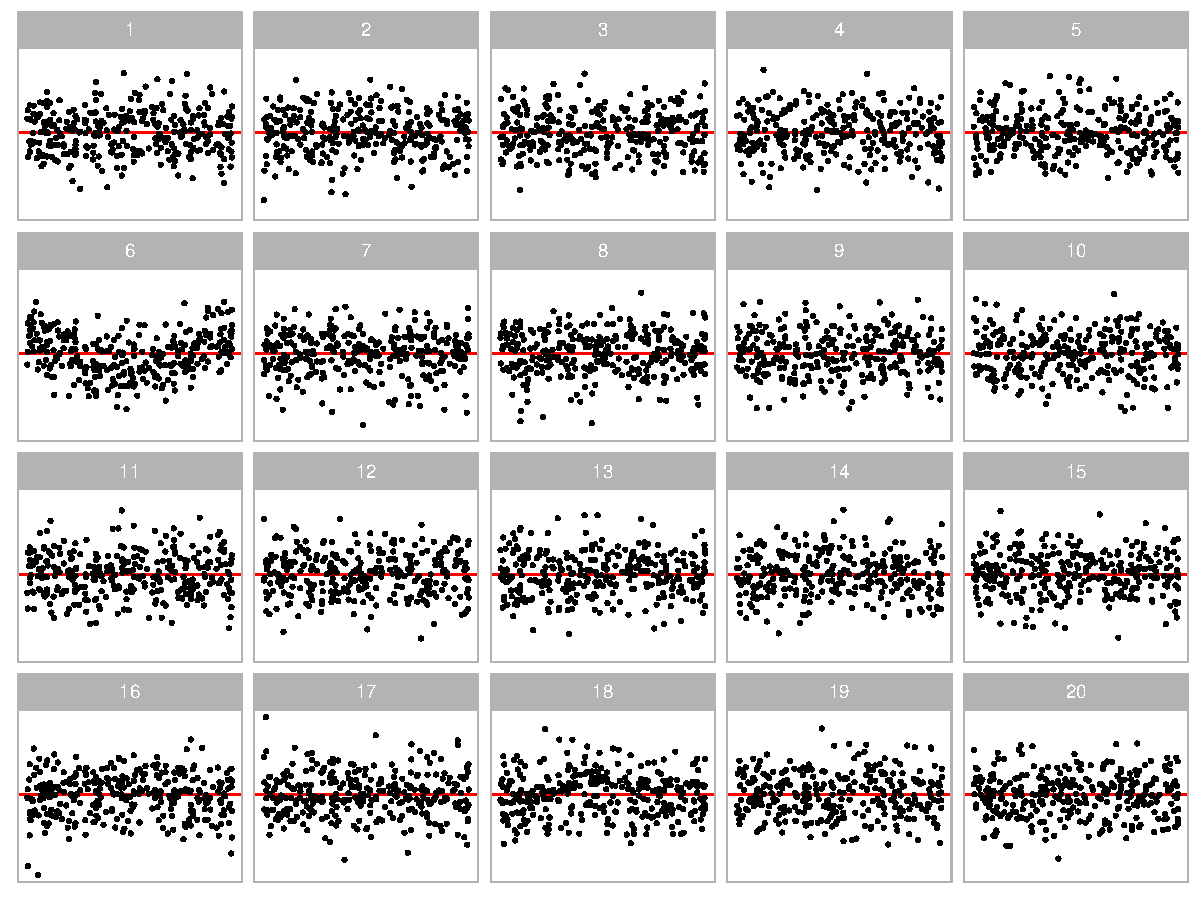
\includegraphics[width=1\linewidth]{paper_comparison_files/figure-latex/first-example-lineup-1} 

}

\caption{Visual testing is conducted using a lineup, as in the example here. The residual plot computed from the observed data (plot $2^2 + 2$, exhibiting non-linearity) is embedded among 19 null plots, where the residuals are simulated from a standard error model. Computing the $p$-value requires that the lineup be examined by a number of human judges, each asked to select the most different plot. A small $p$-value would result from a substantial number selecting plot $2^2 + 2$.}\label{fig:first-example-lineup}
\end{figure}

Figure \ref{fig:first-example-lineup} is an example of a lineup
protocol. If the data plot at position \(2^2 + 2\) is identifiable, then
it is evidence for the rejection of \(H_0\) that the regression model is
correctly specified. In fact, the actual residual plot is obtained from
a misspecified regression model with non-linearity defect.

The effectiveness of lineup protocol for regression analysis is
validated by \citet{majumder_validation_2013} under relatively simple
settings with up to two regressors. Their results suggest that visual
tests are capable of testing the significance of a single regressor with
a similar power as a t-test, though they express that in general it is
unnecessary to use visual inference if there exists a conventional test,
and they do not expect the visual test to perform equally well as the
conventional test. In their third experiment, where there is not a
conventional test, visual test outperforms the conventional test for a
large margin. This is encouraging, as it promotes the use of visual
inference in situations where there are no existing statistical testing
procedures. Visual inference have also been integrated into diagnostic
of hierarchical linear models by \citet{loy2013diagnostic},
\citet{loy2014hlmdiag} and \citet{loy2015you}. They use lineup protocols
to judge the assumption of linearity, normality and constant error
variance for both the level-1 and level-2 residuals. (expand?)

\hypertarget{sampling-from-the-null-distribution}{%
\subsubsection{Sampling from the null
distribution}\label{sampling-from-the-null-distribution}}

Data used in the \(m - 1\) null plots needs to be simulated. In the
context of regression diagnostics, sampling data from \(H_0\) is
equivalent to sampling data from the assumed model. As
\citet{buja_statistical_2009} suggested, \(H_0\) is usually a composite
hypothesis controlled by nuisance parameters. Since regression models
can have various forms, there is no general solution to this problem,
but it sometimes can be reduced to a so called ``reference
distribution'' by applying one of the three methods: (i) sampling from a
conditional distribution given a minimal sufficient statistic under
\(H_0\), (ii) parametric bootstrap sampling with nuisance parameters
estimated under \(H_0\), and (iii) Bayesian posterior predictive
sampling. The conditional distribution given a minimal sufficient
statistic is the best justified reference distribution among the three
\citep{buja_statistical_2009}. Essentially, null residuals can be
simulated by regressing \(N\) i.i.d standard normal random draws on the
regressors, then rescaling it by the ratio of residual sum of square in
two regressions.

\hypertarget{calculating-p-values-for-the-visual-test}{%
\subsubsection{\texorpdfstring{Calculating \(p\)-values for the visual
test}{Calculating p-values for the visual test}}\label{calculating-p-values-for-the-visual-test}}

In hypothesis testing, \(p\)-value is defined as the probability of
observing test results as least as extreme as the observed result given
\(H_0\) is true. Within the context of visual inference, by involving
\(k\) independent observers, \(p\)-value can be interpreted as the
probability of having as many or more subjects detect the data plot than
the observed result.

Let \(X_j = \{0,1\}\) be a binomial random variable denoting whether
subject \(j\) correctly detecting the data plot, and
\(X = \sum_{j=1}^{K}X_j\) be the number of observers correctly picking
the data plot. Then, by imposing a relatively strong assumption on the
visual test that all \(K\) evaluations are fully independent, under
\(H_0\), \(X \sim \mathrm{Binom}_{K,1/m}\). Therefore, the \(p\)-value
of a lineup of size \(m\) evaluated by \(K\) observer is given as
\(P(X \geq x) = 1 - F(x) + f(x)\), where \(F(.)\) is the cumulative
distribution function, \(f(.)\) is the probability mass function and
\(x\) is the realization of number of observers correctly picking the
data plot \citep{majumder_validation_2013}.

As pointed out by \citet{vanderplas2021statistical}, this basic binomial
model doesn't take into account the possible dependencies in the visual
test due to repeated evaluations of the same lineup. And it is
inapplicable to visual test where subjects are asked to select one or
more ``most different'' plots from the lineup.
\citet{vanderplas2021statistical} summarises three common scenarios in
visual inference: (1) \(K\) different lineups are shown to \(K\)
subjects, (2) \(K\) lineups with different null plots but the same data
plot are shown to \(K\) subjects, and (3) the same lineup is shown to
\(K\) subjects. Out of these three scenarios, Scenario 3 is the most
common in previous studies as it puts the least constraints on the
experiment design. For Scenario 3, \citet{vanderplas2021statistical}
models the probability of a plot \(i\) being selected from a lineup as
\(\theta_i\), where \(\theta_i \sim Dirichlet(\alpha)\) for
\(i=1,...,m\) and \(\alpha > 0\). The number of times plot \(i\) being
selected in \(K\) evaluations is denoted as \(c_i\). In case subject
\(j\) makes multiple selections, \(1/s_j\) will be added to \(c_i\)
instead of one, where \(s_j\) is the number of plots subject \(j\)
selected for \(j=1,...K\). This ensures \(\sum_{i}c_i=K\). Since we are
only interested in the selections of the data plot \(i\), the marginal
model can be simplified to a beta-binomial model and thus the visual
p-value is given as

\begin{equation} \label{eq:pvalue-beta-binomial}
P(C \geq c_i) = \sum_{x=c_i}^{K}{K \choose x}\frac{B(x + \alpha, K - x + (m - 1)\alpha)}{B(\alpha, (m-1)\alpha)},\quad \text{for} \quad c_i \in \mathbb{Z}_0^+
\end{equation}

\noindent where \(B(.)\) is the beta function defined as

\begin{equation} \label{eq:betafunction}
B(a, b) = \int_{0}^{1}t^{\alpha - 1}(1-t)^{b-1}dt,\quad \text{where}\quad a,b>0. 
\end{equation}

Note that Equation \ref{eq:pvalue-beta-binomial} given in
\citet{vanderplas2021statistical} only works with non-negative integer
\(c_i\). We extend the equation to non-negative real number \(c_i\) by
applying a linear approximation

\begin{equation} \label{eq:pvalue-beta-binomial-approx}
P(C \geq c_i) = P(C \geq \lceil c_i \rceil) + (\lceil c_i \rceil - c_i) P(C = \lfloor c_i \rfloor), \quad \text{for}\quad c_i \in \mathbb{R}_0^+,
\end{equation}

where \(P(C \geq \lceil c_i \rceil)\) is calculated using Equation
\ref{eq:pvalue-beta-binomial} and \(P(C = \lfloor c_i \rfloor)\) is
calculated by

\begin{equation} \label{eq:pmf-beta-binomial}
P(C = c_i) = {K \choose c_i}\frac{B(c_i + \alpha, K - c_i + (m - 1)\alpha)}{B(\alpha, (m-1)\alpha)},\quad \text{for} \quad c_i \in \mathbb{Z}_0^+.
\end{equation}

Besides, the parameter \(\alpha\) used in Equation
\ref{eq:pvalue-beta-binomial} and \ref{eq:pmf-beta-binomial} is usually
unknown and hence needs to be estimated from the survey data. For low
values of \(\alpha\), only a few plots are attractive to the observers
and tend to be selected. For higher values of \(\alpha\), the
distribution of the probability of each plot being selected is more
even. \citet{vanderplas2021statistical} defines that a plot is
\(c\)-interesting if \(c\) or more participants select the plot as the
most different. Given the definition, The expected number of plots
selected at least \(c\) times, \(E[Z_c]\), is calculated as

\begin{equation} \label{eq:c-interesting-expectation}
E[Z_c(\alpha)] = \frac{m}{B(\alpha, (m-1)\alpha)}\sum_{\lceil c \rceil}^{K}{K \choose x} B(x + \alpha, K - x + (m-1)\alpha).\end{equation}

With Equation \ref{eq:c-interesting-expectation}, \(\alpha\) can be
estimated using maximum likelihood estimation. But for precise estimate
of \(\alpha\), additional responses to Rorschach lineups, which is a
type of lineup that consists of plots constructed from the same null
data generating mechanism, are required.

\hypertarget{power-of-a-visual-test}{%
\subsubsection{Power of a visual test}\label{power-of-a-visual-test}}

The power of a model misspecification test specifies the chance of a
misspecified regression model being detected given a certain alternative
hypothesis. It is an important indicator when one concerns if the
regression model is misspecified. Though, people might usually be more
interested in knowing how much the residuals depart from the model
assumptions and if the departure is of practical significance.

As discussed in \citet{majumder_validation_2013}, individual's skill may
affect the number of observers who identify the data plot from the
lineup. Thus, the power of a visual test could depend on the
subject-specific abilities. Previously, it is addressed by modelling the
probability of a subject \(j\) correctly picking the data plot from a
lineup \(l\) using a mixed-effect logistic regression with the subject
being treated as a random effect \citep{majumder_validation_2013}.
However, in the multiple selections scenario, having this probability is
insufficient to determine the power of a visual test as it doesn't
provide information about the number of selections made by the subject
for p-value calculation.

Instead, we estimate the probability of a lineup being rejected directly
by assuming the individual skill has negligible impact on the variation
of the power of a lineup. The assumption is made to simplify the model
structure, thus mitigating the need for expensive large-scale
experiments to estimate the complex covariance matrix. The model is a
logistic regression with the natural logarithm of the effect as the only
regressor formulated as

\begin{equation} \label{eq:logistic-regression-1-1}
Pr(\text{reject}~H_0|H_1,E) = \Lambda(\beta_0 + \beta_1 log_e(E)),
\end{equation}

\noindent where \(\Lambda(.)\) is the standard logistic function given
as \(\Lambda(z) = exp(z)/(1+exp(z))\).

Effect \(E\) is derived from the Kullback-Leibler divergence (see
{[}appendix ref here{]}) formulated as

\begin{equation} \label{eq:effect-size-ex1}
E = \frac{1}{2\sigma^2}\boldsymbol{X}_b'\boldsymbol{R}_a'(diag(\boldsymbol{R}_a))^{-1}\boldsymbol{R}_a\boldsymbol{X}_b,
\end{equation}

\noindent where \(diag(.)\) is the diagonal matrix constructed from the
diagonal elements of \(\boldsymbol{R}_a\).

To study various factors contributing to the power of the visual test,
the same logistic regression model is fit on different subsets of the
collated data grouped by levels of factors. This includes
{[}expansion{]}.

\hypertarget{experimental-design}{%
\section{Experimental design}\label{experimental-design}}

Three experiments are conducted to investigate the difference between
conventional hypothesis testing and visual inference in the application
of linear regression diagnostics. The experiment I has ideal scenario
for conventional testing, where the visual test is not expected to
outperform the conventional test. Meanwhile, the experiment II is a
scenario where the conventional test is an approximate test, in which
the visual test may have a chance to match the performance of the
conventional test. The experiment III is designed for collecting human
responses to null lineups such that the parameter \(\alpha\) in Equation
\ref{eq:pvalue-beta-binomial} can be estimated. Overall, we plan to
collect 7974 evaluations on 1152 uniqued lineups performed by 443
subjects throughout three experiments.

\hypertarget{simulating-departures-from-good-residuals}{%
\subsection{Simulating departures from good
residuals}\label{simulating-departures-from-good-residuals}}

Two types of departures, namely non-linearity and heteroskedasticity,
are considered with the corresponding data generating process being
designed for experiment I and II.

\hypertarget{non-linearity}{%
\subsubsection{Non-linearity}\label{non-linearity}}

\begin{figure}

{\centering 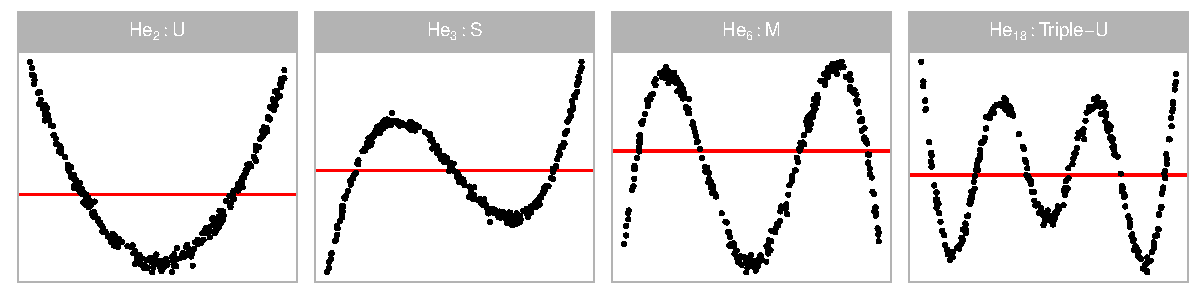
\includegraphics[width=1\linewidth]{paper_comparison_files/figure-latex/different-shape-of-herimite-1} 

}

\caption{Polynomial forms generated for the residual plots used in experiment I. The four shapes are generated by varying the order of polynomial given by $j$ in $He_j(.)$.}\label{fig:different-shape-of-herimite}
\end{figure}

Experiment I is designed to study the ability of human subjects to
detect the effect of a non-linear term \(\boldsymbol{z}\) constructed
using Hermite polynomials on random vector \(\boldsymbol{x}\) formulated
as

\begin{align} \label{eq:nonlinearity-model}
\boldsymbol{y} = 1 + \boldsymbol{x} + \boldsymbol{z} + \boldsymbol{\varepsilon},\\
\boldsymbol{x} = g(\boldsymbol{x}_{raw}, 1), \\
\boldsymbol{z} = g(\boldsymbol{z}_{raw}, 1), \\
\boldsymbol{z}_{raw} = He_j(g(\boldsymbol{x}, 2)),
\end{align}

\noindent where \(\boldsymbol{y}\), \(\boldsymbol{x}\),
\(\boldsymbol{\varepsilon}\), \(\boldsymbol{x}_{raw}\),
\(\boldsymbol{z}_{raw}\) are vectors of size \(n\), \(He_{j}(.)\) is the
\(j\)th-order probabilist's Hermite polynomials,
\(\varepsilon \sim N(\boldsymbol{0}, \sigma^2\boldsymbol{I}_n)\), and
\(g(\boldsymbol{x}, k)\) is a scaling function to enforce the support of
the random vector to be \([-k, k]^n\) defined as

\begin{equation} \label{eq:scaling-function}
g(\boldsymbol{x}, k) = (\boldsymbol{x} - min(\boldsymbol{x}))/max(\boldsymbol{x} - min(\boldsymbol{x}))2k - k, \quad \text{for} \quad k > 0. 
\end{equation}

According to \citet{abramowitz1964handbook}, Hermite polynomials were
initially defined by \citet{de1820theorie}, but named after Hermite
\citep{hermite1864nouveau} because of the unrecognisable form of
Laplace's work. When simulating \(\boldsymbol{z}_{raw}\), function
\texttt{hermite} from the R package \texttt{mpoly} \citep{mpoly} is used
to generate Hermite polynomials.

The null regression model used to fit the realizations generated by the
above model is formulated as

\begin{equation} \label{eq:null-model}
\boldsymbol{y} = \beta_0 + \beta_1 \boldsymbol{x} + \boldsymbol{u},
\end{equation}

\noindent where
\(\boldsymbol{u} \sim N(\boldsymbol{0}, \sigma^2\boldsymbol{I}_n)\).

Since \(z = O(x^j)\), for \(j > 1\), \(z\) is a higher order term leaves
out by the null regression, which will lead to model misspecification.

Visual patterns of non-linearity are simulated using four different
orders of probabilist's Hermite polynomials (\(j = 2, 3, 6, 18\)) and
four different distributions of \(X_{raw}\): (1) \(U(-1, 1)\), (2)
\(N(0, 0.3^2)\), (3) \(lognormal(0, 0.6^2)/3\) and (4) \(u\{1, 5\}\). A
summary of the factors is given in Table \ref{tab:model-factor-table}.

\begin{table}

\caption{\label{tab:model-factor-table}Description of all factors involved in the non-linear and heteroskedasticity studies.}
\centering
\resizebox{\linewidth}{!}{
\begin{tabular}[t]{rcrrrr}
\toprule
\multicolumn{1}{c}{Poly Order ($j$)} & \multicolumn{1}{c}{\makecell[c]{Distribution of $X_{raw}$\\}} & \multicolumn{1}{c}{SD ($\sigma$)} & \multicolumn{1}{c}{Heteroskedasticity Shape ($a$)} & \multicolumn{1}{c}{Heteroskedasticity ($b$)} & \multicolumn{1}{c}{Size ($n$)} \\
\cmidrule(l{3pt}r{3pt}){1-1} \cmidrule(l{3pt}r{3pt}){2-2} \cmidrule(l{3pt}r{3pt}){3-3} \cmidrule(l{3pt}r{3pt}){4-4} \cmidrule(l{3pt}r{3pt}){5-5} \cmidrule(l{3pt}r{3pt}){6-6}
2 & $U(-1, 1)$ & 0.25 & -1 & 0.25 & 50\\
3 & $N(0, 0.3^2)$ & 1.00 & 0 & 1.00 & 100\\
6 & $lognormal(0, 0.6^2)/3$ & 2.00 & 1 & 4.00 & 300\\
18 & $U\{1, 5\}$ & 4.00 &  & 16.00 & \\
 &  &  &  & 64.00 & \\
\bottomrule
\end{tabular}}
\end{table}

The values of \(j\) is chosen so that distinct shapes of non-linearity
are included in the residual plot. These include ``U'', ``S'', ``M'' and
``Triple-U'' shape as shown in Figure
\ref{fig:different-shape-of-herimite}. A greater value of \(j\) will
result in a curve with more turning points. It is expected that the
``U'' shape will be the easiest one to detect because complex shape
tends to be concealed by cluster of data points.

Different distributions of \(X_{raw}\) help enriching the pool of visual
patterns as illustrated in Figure \ref{fig:different-dist}. The uniform
and the normal distribution are symmetric and commonly assumed in
statistical models. The adjusted log-normal distribution provides skewed
density, while the discrete uniform distribution provides discreteness
in residual plot.

\begin{figure}

{\centering 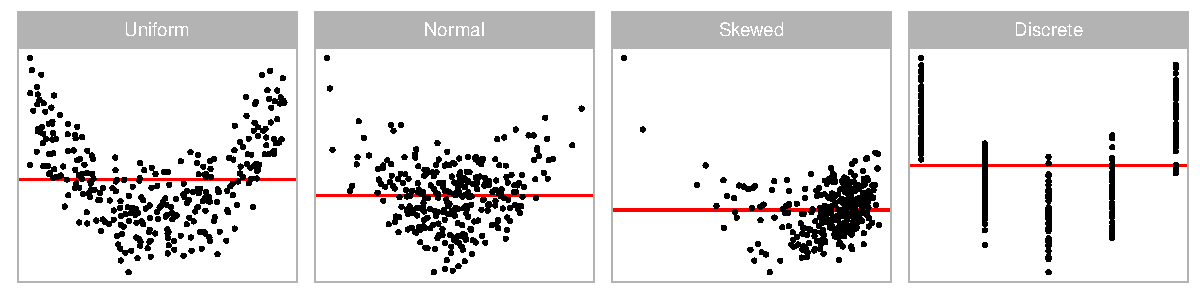
\includegraphics[width=1\linewidth]{paper_comparison_files/figure-latex/different-dist-1} 

}

\caption{Variations in fitted values, that might affect perception of residual plots. Four different distribution of $X_{raw}$ are used in the experiment to provide various visual patterns.}\label{fig:different-dist}
\end{figure}

Figure \ref{fig:example-poly-lineup} demonstrates one of the lineups
used in experiment I. This lineup is produced by the non-linearity model
under \(j = 6\) and \(X_{raw} \sim N(0.0.3^2)\). The data plot location
is \(2^3 - 4\). All five subjects correctly identify the data plot from
this lineup.

\begin{figure}

{\centering 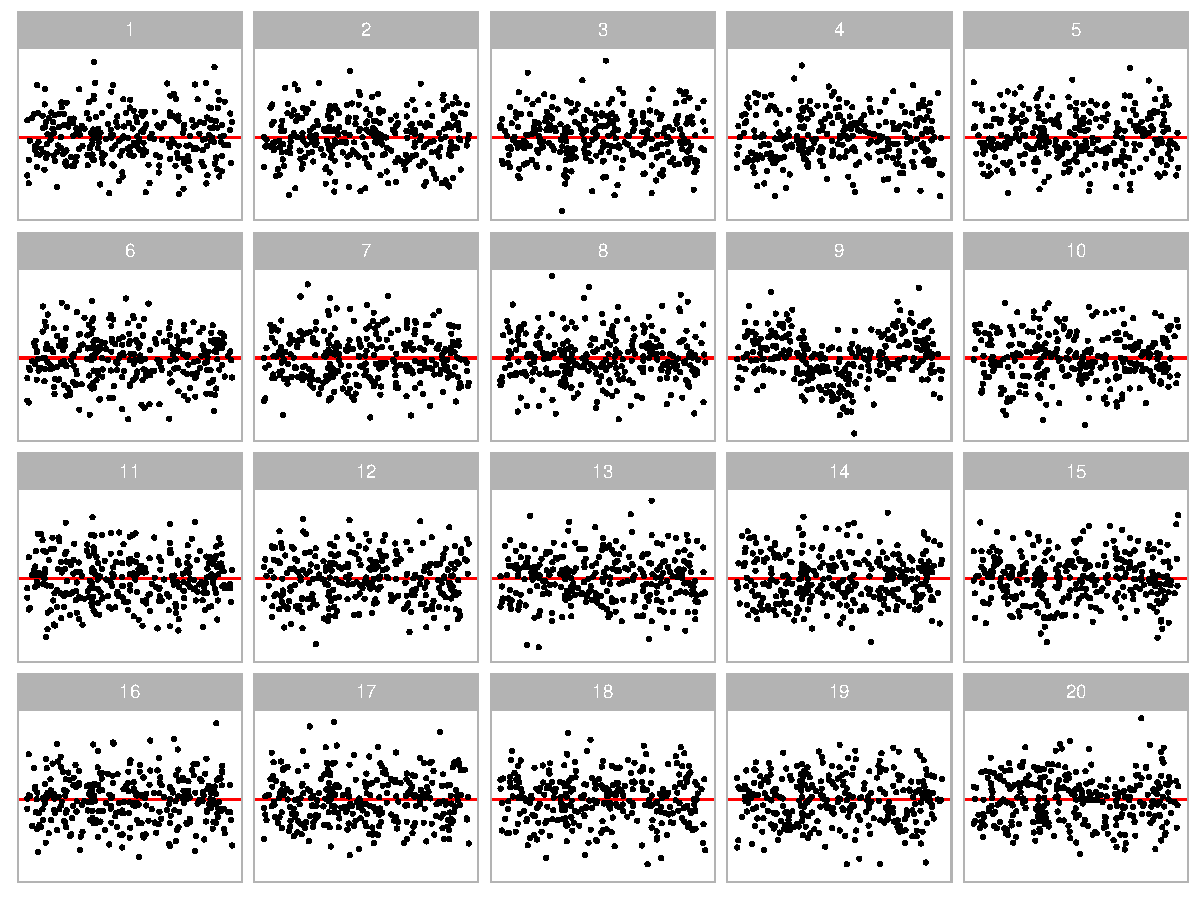
\includegraphics[width=1\linewidth]{paper_comparison_files/figure-latex/example-poly-lineup-1} 

}

\caption{Lineup poly-24 in experiment I. Can you spot the most different plot? \label{fig:example-poly-lineup}}\label{fig:example-poly-lineup}
\end{figure}

\hypertarget{heteroskedasticity}{%
\subsubsection{Heteroskedasticity}\label{heteroskedasticity}}

Experiment II is designed to study the ability of human subjects to
detect the appearance of a heteroskedasticity pattern under a simple
linear regression model setting:

\begin{align} \label{eq:heter-model}
\boldsymbol{y} = 1 + \boldsymbol{x} + \boldsymbol{\varepsilon},\\
\boldsymbol{x} = g(\boldsymbol{x}_{raw}, 1)\\
\boldsymbol{\varepsilon} \sim N(\boldsymbol{0}, 1 + (2 - |a|)(\boldsymbol{x} - a)^2b \boldsymbol{I}), \\
\end{align}

\noindent where \(\boldsymbol{y}\), \(\boldsymbol{x}\),
\(\boldsymbol{\varepsilon}\) are vectors of size \(n\) and \(g(.)\) is
the scaling function defined in Equation \ref{eq:scaling-function}.

The null regression model used to fit the realizations generated by the
above model is formulated exactly the same as Equation
\ref{eq:null-model}.

For \(b \neq 0\), the variance-covariance matrix of the error term
\(\boldsymbol{\varepsilon}\) is correlated with the regressor
\(\boldsymbol{x}\), which will lead to the presence of
heteroskedasticity. Visual patterns of heteroskedasticity are simulated
using three different shapes (\(a\) = -1, 0, 1) and the same four
different distribution of \(X_{raw}\) used in experiment I. A summary of
the factors can also be found in Table \ref{tab:model-factor-table}.

Since \(supp(X) = [-1, 1]\), choosing \(a\) to be \(-1\), \(0\) and
\(1\) can generate ``left-triangle'', ``butterfly'' and
``right-triangle'' shape as displayed in Figure
\ref{fig:different-shape-of-heter}. The term \((2 - |a|)\) maintains the
magnitude of residuals across different values of \(a\).

\begin{figure}

{\centering 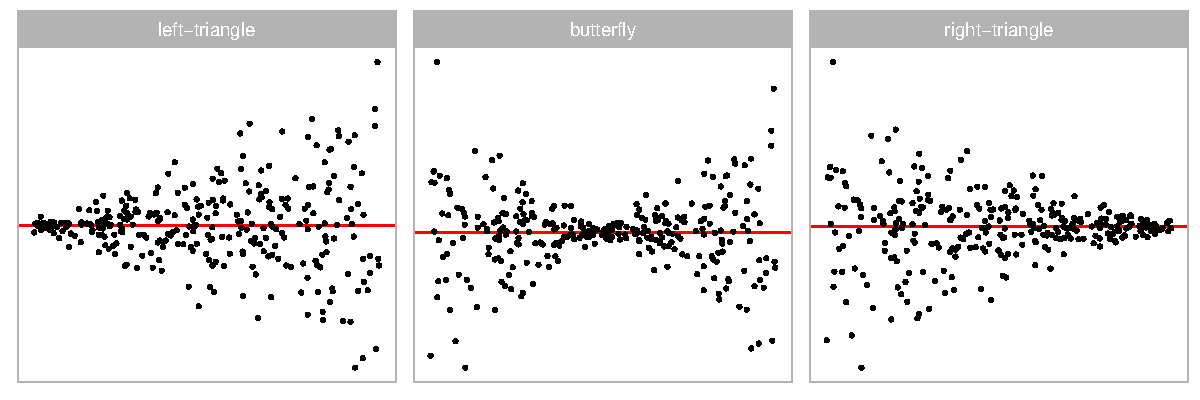
\includegraphics[width=1\linewidth]{paper_comparison_files/figure-latex/different-shape-of-heter-1} 

}

\caption{Heteroskedasticity forms used in experiment II. Three different shapes (a = -1, 0, 1) are used in the experiment to create left-triangle, butterfly and right-triangle shapes.}\label{fig:different-shape-of-heter}
\end{figure}

\begin{figure}

{\centering 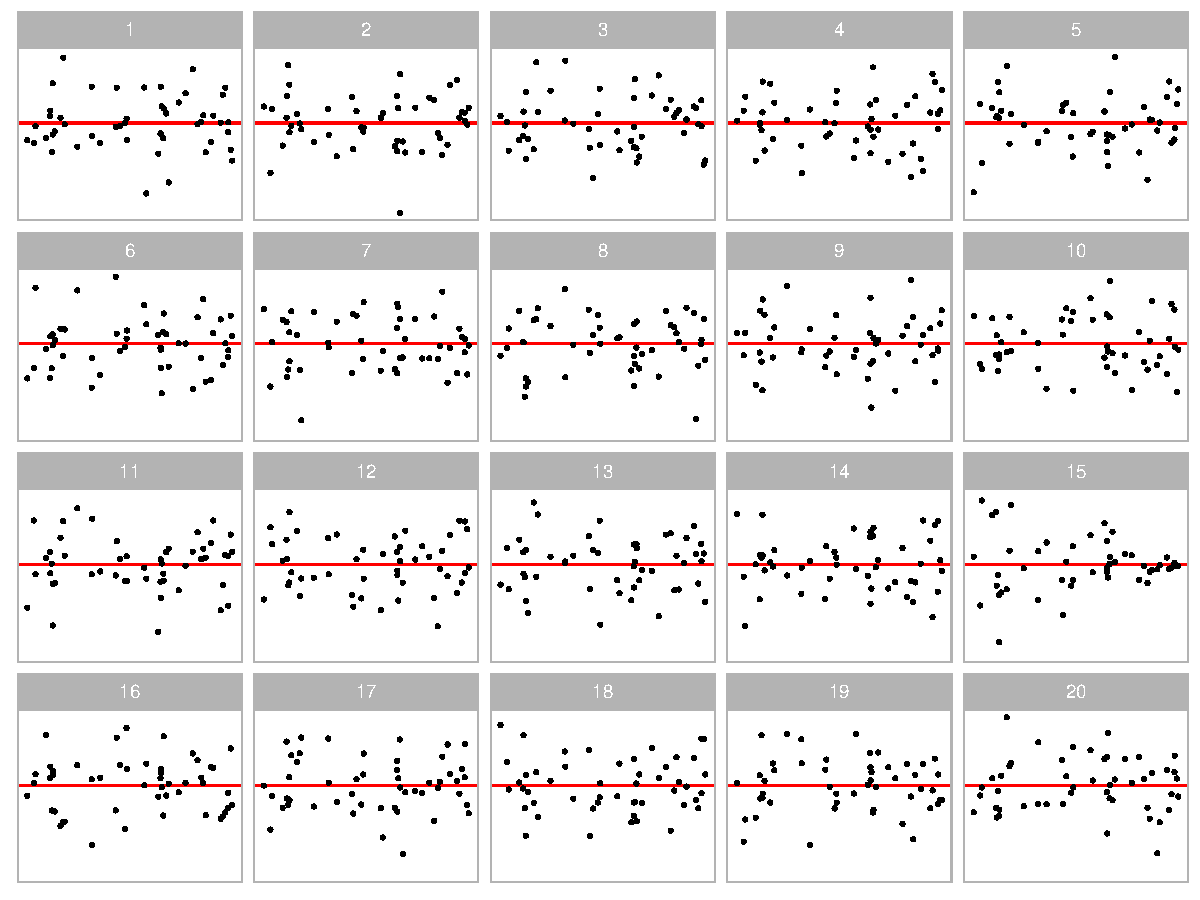
\includegraphics[width=1\linewidth]{paper_comparison_files/figure-latex/example-heter-lineup-1} 

}

\caption{Lineup heter-169 in experiment II. Can you spot the most different plot? \label{fig:example-heter-lineup}}\label{fig:example-heter-lineup}
\end{figure}

An example lineup of this model used in Experiment II is shown in Figure
\ref{fig:example-heter-lineup} with \(a = -1\) and
\(X_{raw} \sim U(-1, 1)\). The data plot location is \(2^4 + 2\). Nine
out of 11 subjects correctly identify the data plot from this lineup.

\hypertarget{experimental-setup}{%
\subsection{Experimental setup}\label{experimental-setup}}

\hypertarget{controlling-the-strength-of-the-signal}{%
\subsubsection{Controlling the strength of the
signal}\label{controlling-the-strength-of-the-signal}}

As summarised in Table \ref{tab:model-factor-table}, three additional
parameters \(n\), \(\sigma\) and \(b\) are used to control the strength
of the signal so that different difficulty levels of lineups are
generated, and therefore, the estimated power curve will be smooth and
continuous. Parameter \(\sigma \in \{0.5, 1, 2, 4\}\) and
\(b \in \{0.25, 1, 4, 16, 64\}\) are used in experiment I and II
respectively. Figure \ref{fig:different-sigma} and \ref{fig:different-b}
demonstrate the impact of these two parameters. A large value of
\(\sigma\) will increase the variation of the error of the non-linearity
model and decrease the visibility of the visual pattern. The parameter
\(b\) controls the standard deviation of the error across the support of
the regressor. Given \(x \neq a\), a larger value of \(b\) will lead to
a larger ratio of the variance at \(x\) to the variance at
\(x - a = 0\), making the visual pattern more obvious.

Three different sample sizes are used (n = 50, 100, 300) in all three
experiments. It can be observed from Figure \ref{fig:different-n} that
with fewer data points drawn in a residual plot, the visual pattern is
more difficult to be detected.

\begin{figure}

{\centering 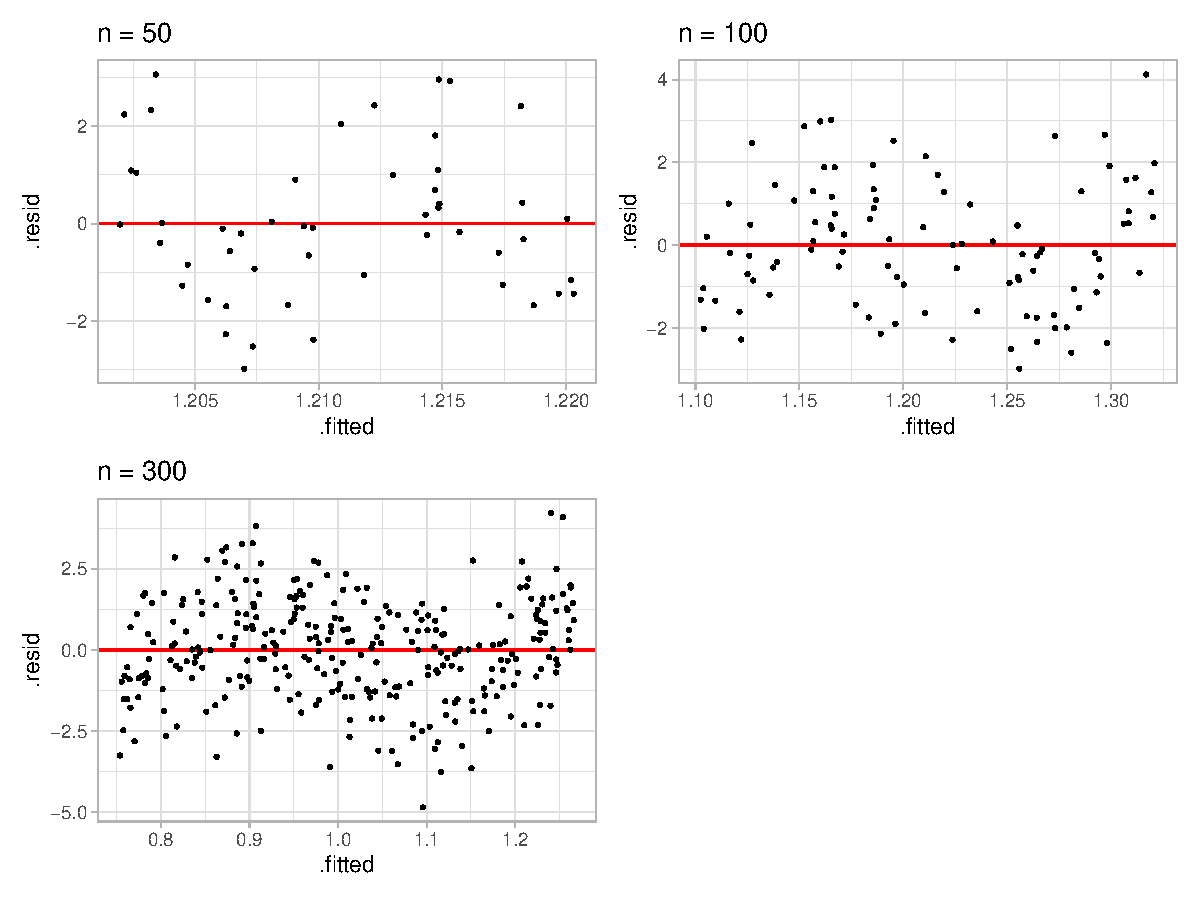
\includegraphics[width=1\linewidth]{paper_comparison_files/figure-latex/different-n-1} 

}

\caption{Three different values of $n$ are used in experiment I, II and III to control the strength of the signal.}\label{fig:different-n}
\end{figure}

\begin{figure}

{\centering 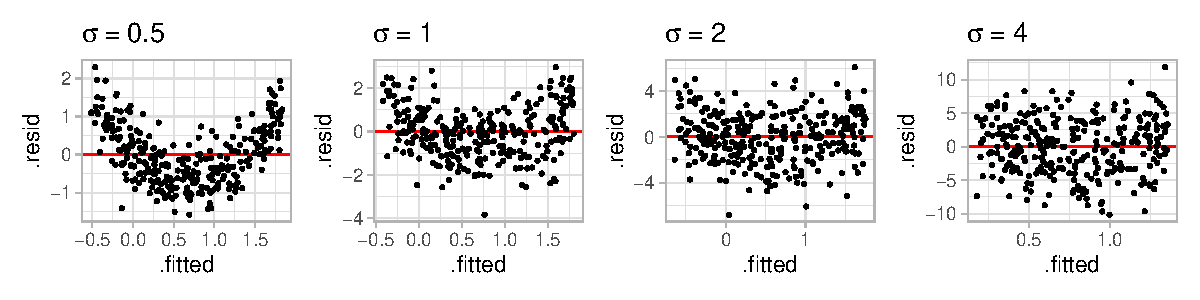
\includegraphics[width=1\linewidth]{paper_comparison_files/figure-latex/different-sigma-1} 

}

\caption{Four different values of $\sigma$ are used in the experiment I to control the strength of the signal.}\label{fig:different-sigma}
\end{figure}

\begin{figure}

{\centering 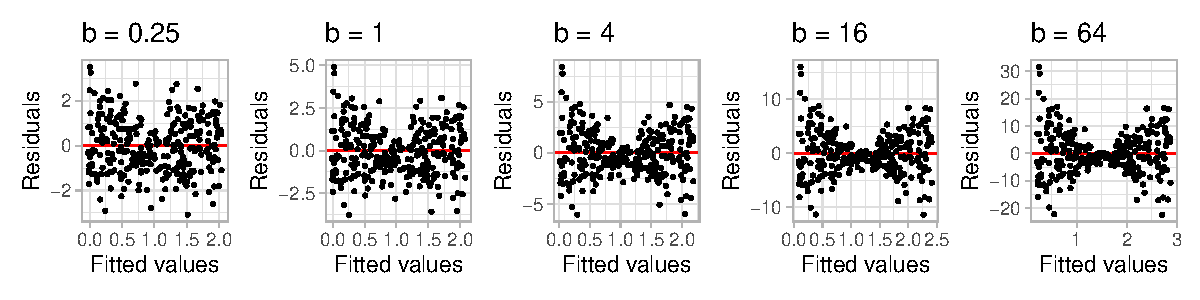
\includegraphics[width=1\linewidth]{paper_comparison_files/figure-latex/different-b-1} 

}

\caption{Five different values of $b$ are used in experiment II to control the strength of the signal.}\label{fig:different-b}
\end{figure}

\hypertarget{subject-allocation}{%
\subsubsection{Subject allocation}\label{subject-allocation}}

Three replications are made for each of the parameter values shown in
Table \ref{tab:model-factor-table} resulting in
\((4 \times 4 \times 4 \times 3 + 4 \times 3 \times 5 \times 3) \times 3 = 1116\)
different lineups. In addition, each lineup is designed to be evaluated
by five different subjects. After attempting some pilot studies
internally in our research group, we decide to present a block of 20
lineups to every subject. And to ensure the quality of the survey data,
two lineups with obvious visual patterns are included as attention
checks. Thus, \(576 \times 5 / (20-2) = 160\) and
\(540 \times 5 / (20-2) = 150\) subjects are recruited to satisfy the
design of the experiment I and experiment II respectively.

As mentioned in Section \ref{calculating-p-values-for-the-visual-test},
\(\alpha\) used in Equation \ref{eq:pvalue-beta-binomial} needs to be
estimated using {\textcolor{orange-red}{null}} lineups. Hence, 36
lineups with all combinations of \(n\) and \(X_{raw}\) and three
replications are included in experiment III. In these lineups, the data
of the data plot is generated from a model
{\textcolor{orange-red}{with zero effect size}}, while the data of the
19 null plots are generated using the same simulation method discussed
in Section \ref{sampling-from-the-null-distribution}.
{\textcolor{orange-red}{This generation procedure differs from the canonical Rorschach lineup procedure, which requires that all 20 plots are generated from the null hypothesis. However, these lineups serve the same fundamental purpose: to assess the number of visually interesting plots generated under the null hypothesis.}}
{\textcolor{orange-red}{To account for the fact that our simulation method for these lineups is not the Rorschach procedure,}}
we use the method suggested in \citet{vanderplas2021statistical} for
typical lineups containing a data plot to estimate \(\alpha\). We have
included a sensitivity analysis in the Appendix to examine the impact of
the variance of the \(\alpha\) estimate on our findings.

All lineups consist of only null plots are planned to be evaluated by 20
subjects. However, presenting only these lineups to subjects are
considered to be bad practices as subjects will lose interest quickly.
Therefore, we plan to collect 6 more evaluations on the 279 lineups with
\(X_{raw} \sim U(-1,1)\), result in
\((36 \times 20 + (4 \times 4 \times 3 + 3 \times 5 \times 3) \times 3) / (20-2) = 133\)
subjects recruited for experiment III.

\hypertarget{collecting-results}{%
\subsubsection{Collecting results}\label{collecting-results}}

Subjects for all three experiments are recruited from an crowdsourcing
platform called Prolific \citep{palan2018prolific}. Prescreening
procedure is applied during the recruitment, subjects are required to be
fluent in English, with \(98\%\) minimum approval rate and 10 minimum
submissions in other studies.

During the experiment, every subject is presented with a block of 20
lineups. A lineup consists of a randomly placed data plot and 19 null
plots, which are all residual plots drawn with raw residuals on the
y-axis and fitted values on the x-axis. An additional horizontal red
line is added at \(y = 0\) as a helping line.

The data of the data plot is simulated from one of two models described
in Section \ref{simulating-departures-from-good-residuals}, while the
data of the remaining 19 null plots are generated by the residual
rotation technique discussed in Section
\ref{sampling-from-the-null-distribution}.

In every lineup evaluation, the subject is asked to select one or more
plots that are most different from others, provide a reason for their
selections, and evaluate how different they think the selected plots are
from others. If there is no noticeable difference between plots in a
lineup, subjects are permitted to select zero plots without providing
the reason. No subject are shown the same lineup twice. Information
about preferred pronoun, age group, education, and previous experience
in visual experiment are also collected. A subject's submission is only
accepted if the data plot is identified for at least one attention
check. Data of rejected submissions are discarded automatically to
maintain the overall data quality.

\hypertarget{results}{%
\section{Results}\label{results}}

\hypertarget{overview}{%
\subsection{Overview}\label{overview}}

There are 2880, 2700 and 2394 lineups evaluation made by 160, 150 and
133 subjects recruited for experiment I, II and III respectively. In the
total of 7974 lineup evaluations, 3744 use lineups produced by the
non-linearity model, 3510 use lineups produced by the heteroskedasticity
model, and 720 use null lineups. Besides, there are 886 attention checks
not included in the following analysis. The collated dataset is provided
in \texttt{vi\_survey} of the \texttt{visage} \texttt{R} package.

\hypertarget{comparison-of-the-power-of-different-tests}{%
\subsection{Comparison of the power of different
tests}\label{comparison-of-the-power-of-different-tests}}

Figure \ref{fig:polypower} shows the estimated power of visual test on
lineups produced by the non-linearity model with
\(X_{raw} \sim U(-1,1)\), against the natural logarithm of the effect
\(log_e(E)\), with a 5\% significance level. Uniform distribution is the
focus of this section because visual patterns are more likely to be
revealed. Besides, six more evaluations are collected for the uniform
distribution in experiment III, which will produce more reliable and
stable power curves. Analysis of other distributions can be found in
Section \ref{effect-of-the-distribution-of-the-regressor}. At the bottom
of the figure \ref{fig:polypower}, there are a sequence of example
residual plots with increasing levels of \(log_e(E)\). Readers can
evaluate them from left to right and determine at which level the
departure from a good residual plot becomes detectable.

As discussed in Section \ref{conventionally-testing-for-departures},
many conventionally tests are available for detecting residual
departures. Implementation-wise, the built-in R package \texttt{stats}
provides some commonly used residual-based tests, such as Shapiro-Wilk
test. A more comprehensive collection of regression diagnostics tests
can be found in the R package \texttt{lmtest} \citep{lmtest}. In terms
of heteroskedasticity diagnostics, the R package \texttt{skedastic}
\citep{skedastic} collects and implements 25 existing conventional tests
published since 1961.

To compare the power of visual test and conventional test, we pick RESET
test (\texttt{resettest}) and Breusch-Pagan test (\texttt{bptest}) from
the R package \texttt{lmtest}, and Shapiro-Wilk test
(\texttt{shapiro.test}) from the built-in R package \texttt{stats}.
Among them, RESET test is the only exact and appropriate test in this
scenario. Both the Breusch-Pagan test and the Shapiro-Wilk test are
approximate and inappropriate tests. Their estimated power is shown in
Figure \ref{fig:polypower}. To set up the RESET test, we include
different powers of fitted values as proxies. According to
\citet{ramsey_tests_1969}, there are no general rules for the power of
the fitted values needed by the RESET test, but it finds power up to
four is usually sufficient. Thus, we follow this guideline to conduct
the RESET test. For the Breusch-Pagan test, the choice of regressors in
the auxiliary regression is left to the user
\citep{breusch_simple_1979}. But as \citet{waldman1983note} suggested,
it is a good choice for the set of auxiliary regressors in the
Breusch-Pagan test be the same as the White test. Thus, we include both
\(\boldsymbol{x}\) and \(\boldsymbol{x}^2\) in the auxiliary regression.

Figure \ref{fig:heterpower} is similar to Figure \ref{fig:polypower},
but shows corresponding information on lineups produced by the
heteroskedasticity model. In this scenario, the visual test is compared
to an approximate test - Breusch-Pagan test, and two other inappropriate
tests - RESET test and Shapiro-Wilk test.

For the non-linearity model, the power curve of RESET test climbs
aggressively from 13\% to around 70\% as \(log_e(E)\) increases from 0
to 2, while power of other tests respond inactively to the change of
effect, showing that REST test is way more sensitive to the type of
model defects that being considered. Meanwhile, no noticeable visual
features can be spotted from the example residual plots.

In terms of the heteroskedasticity model, the power of Breusch-Pagan
test is also almost always greater than the power of visual test. For
\(0 \leq log_e(E) \leq 2\), where the power curve of the visual test
remains at a low level, the Breusch-Pagan test still have a decent
amount of chance of rejecting \(H_0\). Similarly, the visual feature is
nearly unobservable from the example residual plots.

The power of visual test arises steadily as \(log_e(E)\) increases from
2 to 5 for both non-linearity model and heteroskedasticity model,
suggesting that the effect starts to make significant impact on the
degree of the presence of the designed visual features. This can also be
observed from the example residual plots that when \(log_e(E) = 2.5\), a
weak ``S-shape'' and a weak ``triangle'' shape are presented in Figure
\ref{fig:polypower} and Figure \ref{fig:heterpower} respectively. The
visual pattern becomes much clearer as \(log_e(E)\) increases. At
\(log_e(E) \approx 6\), the power reaches almost 100\%.

The power of all inappropriate tests except for RESET test shows
improvement as the effect increases but at a lower rate than the visual
test in both scenarios. This coincides the point made by
\citet{cook1982residuals} that residual-based tests for a specific type
of model defect may be sensitive to other types of model defects. The
power curve of RESET test remains at around 5\% in Figure
\ref{fig:heterpower} since there are no non-linear terms leave out in
the heteroskedasticity model and \(H_0\) of the test is always
satisfied.

Overall, the power comparison suggests that conventional tests differs
significantly from visual tests in two regression diagnostics scenarios
designed by us. Visual test have much higher tolerance of the residual
departures than the conventional test. Since fail to reject \(H_0\) in a
visual test usually means that there are no obvious visual discoveries
found in the residual plot, analysts and the general public as the
consumers of the output may not be convinced of the existence of
significant residual departures in spite of the rejection of \(H_0\)
given by the conventional test. Even if the rejection is accepted, the
model violation may be considered as impactless due to the fact that
they are not clearly visible. Besides, the sensitivity of the
conventional test could also distract and discourage analysts from
finding simple but good linear approximation to the data. The rejection
of \(H_0\) because of human acceptable and negligible residual
departures is not practically meaningful and useful. This may limit the
popularity of conventional tests in residual diagnostics among analysts.

\begin{figure}

{\centering 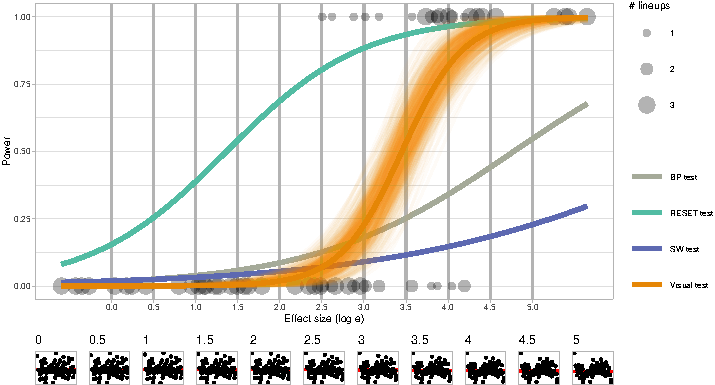
\includegraphics[width=1\linewidth]{paper_comparison_files/figure-latex/polypower-1} 

}

\caption{Comparison of power between different tests for non-linear patterns. Main plot shows the power curves, with dots indicating human evaluations of lineups. Small row of plots shows typical residual plots corresponding to specific effect sizes, marked by dashed lines in main plot. Where would you draw the line of too much non-linearity in the residuals? For the RESET test this is around log effect size 1.5, but for the visual test it is around 3.5.}\label{fig:polypower}
\end{figure}

\begin{figure}

{\centering 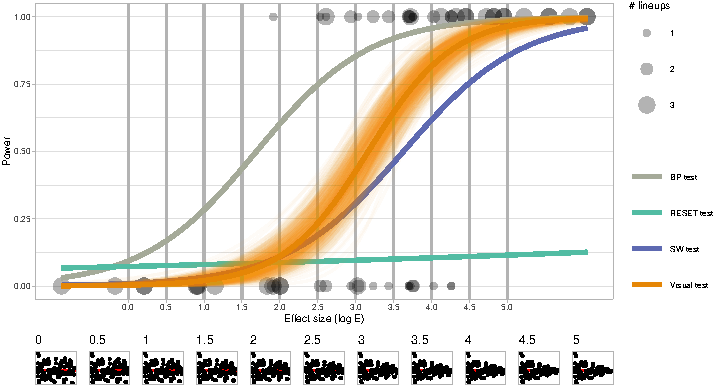
\includegraphics[width=1\linewidth]{paper_comparison_files/figure-latex/heterpower-1} 

}

\caption{Comparison of power between different tests for heteroskedasticity patterns. Main plot shows the power curves, with dots indicating human evaluations of lineups. Small row of plots shows typical residual plots corresponding to specific effect sizes, marked by dashed lines in main plot. Where would you draw the line of too much heteroskedasticity in the residuals? For the BP test this is around log effect size 1.5, but for the visual test it is around 3.}\label{fig:heterpower}
\end{figure}

\hypertarget{comparison-of-rejection-rates-based-on-p-values}{%
\subsection{\texorpdfstring{Comparison of rejection rates based on
\(p\)-values}{Comparison of rejection rates based on p-values}}\label{comparison-of-rejection-rates-based-on-p-values}}

The power comparison illustrates that appropriate conventional tests
reject \(H_0\) more aggressively than visual tests. In this section, we
explore how often they agree with each other by investigate the
rejection rates based on \(p\)-values.

Depending on the natural logarithm of the effect, lineups are classified
into three categories: easy (\textgreater{} 3.5), moderate (1.5 - 3.5)
and difficult (\textless{} 1.5). Figure \ref{fig:p-value-comparison}
provides a mosaic plot showing the rejection rate of visual tests and
conventional tests at different difficulty levels.

\hypertarget{easy-lineup}{%
\subsubsection{Easy lineup}\label{easy-lineup}}

For easy lineups produced by the non-linearity model, 65\% are rejected
by both the conventional and visual tests, while 9\% are accepted by
both tests. Thus, 74\% of the time two tests will agree with each other.
There are 16\% of lineups rejected by conventional tests only.

Interestingly, in spite of the greater power of conventional tests, 10\%
of the lineups are rejected by visual tests only. Recall that the RESET
test used in our analysis includes powers of fitted values up to four.
However, the ``M'' and the ``Triple-U'' shapes constructed from the
Hermite polynomials contain power of the regressor up to six and 18
respectively. In fact, by including the power of fitted values up to six
in the RESET test, all these cases will be rejected. We also can observe
from the example plot displayed in Figure \ref{fig:easy-poly-example}
that panel three is distinctly different from others, exhibiting a ``M''
shape. This clearly suggests users of the RESET test and any other
residual-based conventional tests that require the specification of
variables of interest to check the residual plot before conducting the
test, such that the correct choice of variables can be made.

\begin{figure}

{\centering 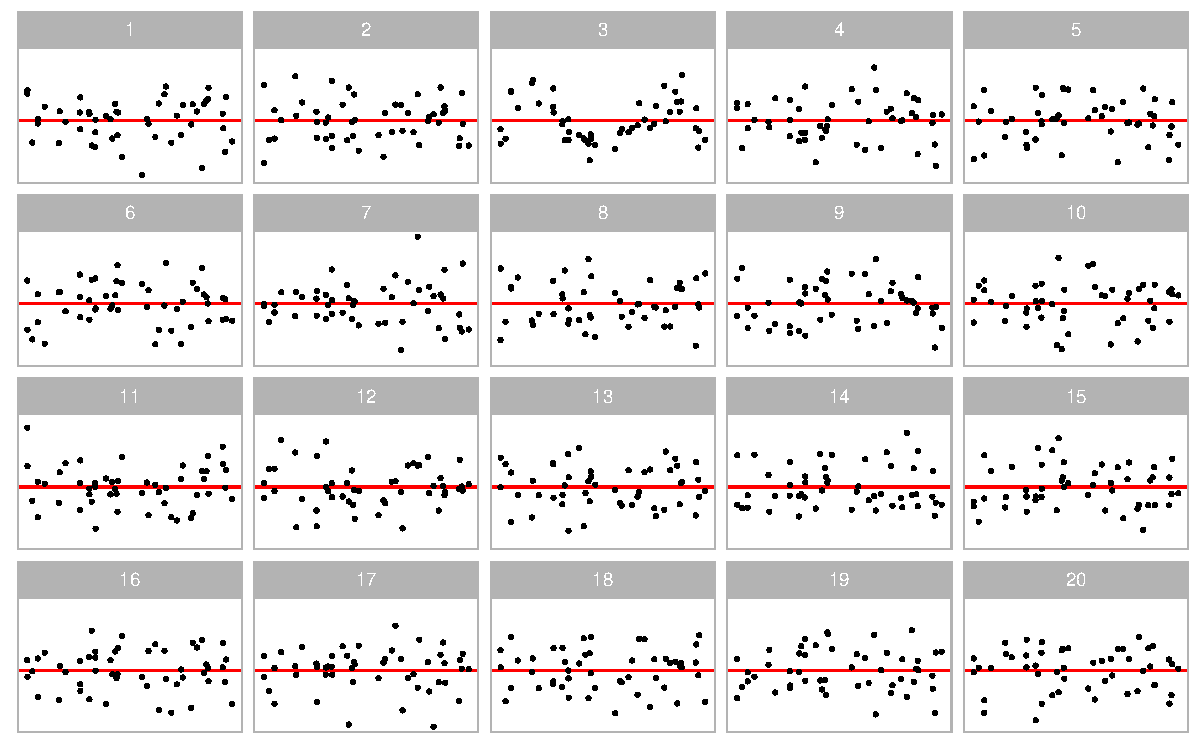
\includegraphics[width=1\linewidth]{paper_comparison_files/figure-latex/easy-poly-example-1} 

}

\caption{Lineup poly-270 with $log_e(E) = 3.89$ produced by the non-linearity model used in experiment I and III. It is rejected by the visual test but not by the RESET test. The data plot at panel three exhibits strong non-linear pattern.}\label{fig:easy-poly-example}
\end{figure}

For easy lineups produced by the heteroskedasticity model, 62\% are
rejected by both the conventional test and the visual test, and 7\% are
accepted by both, result in 69\% agreement rate. Lineups only rejected
by conventional test are 30\%. 1\% of lineups are accepted by the
conventional test but rejected by the visual test.

Among those 1\%, which are two lineups, one shows detectable
heteroskedasticity pattern as displayed in Figure
\ref{fig:easy-heter-example1}. Another contain data plot with an
noticeable outlier, but the ``Right-triangle'' shape is not very strong
as shown in Figure \ref{fig:easy-heter-example2}. The \(p\)-values of
Breusch-Pagan test for these two lineups are \(0.055\) and \(0.135\).
Compared to the visual test, its \(p\)-values are \(0.026\) and
\(0.012\). The Breusch-Pagan test should reject the one with obvious
heteroskedasticity signal, but it yields a \(p\)-value slightly above
5\%.

\begin{figure}

{\centering 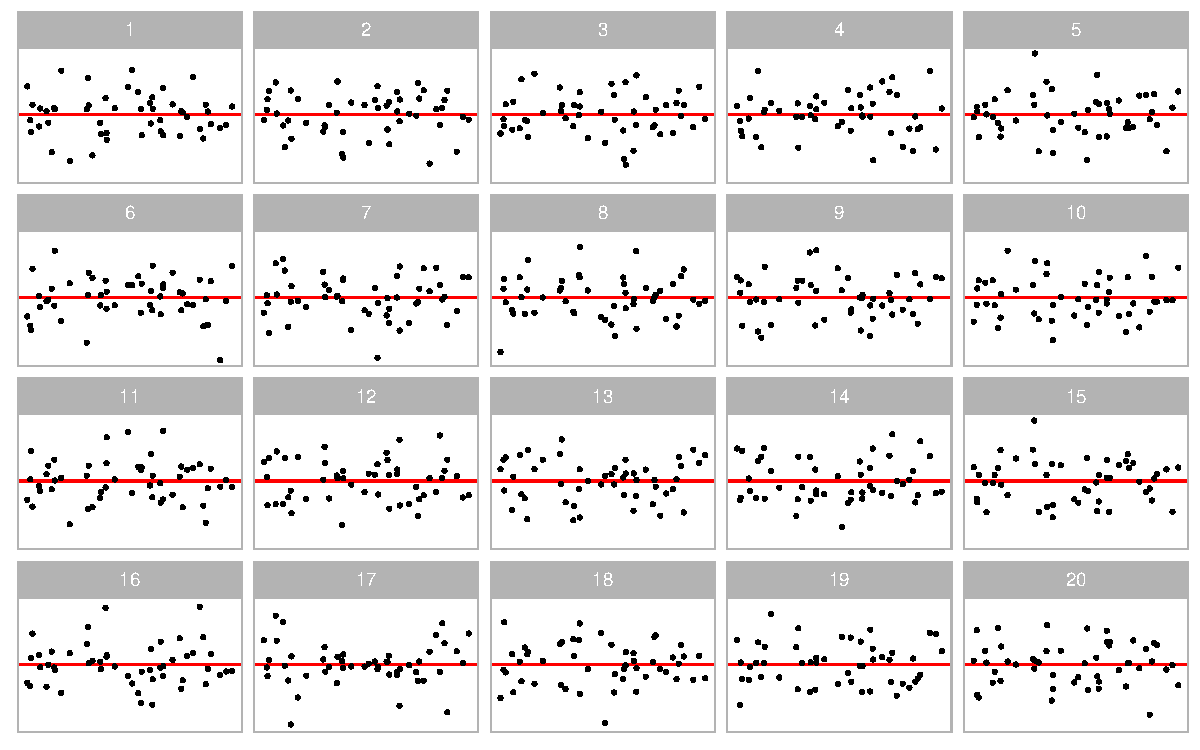
\includegraphics[width=1\linewidth]{paper_comparison_files/figure-latex/easy-heter-example1-1} 

}

\caption{Lineup heter-331 with $log_e(E) = 4.02$ produced by the heteroskedasticity model used in experiment II and III. It is rejected by the visual test but not by the  Breusch-Pagan test. The data plot at panel 17 contains a "Butterfly" shape, indicating the presence of heteroskedasticity.}\label{fig:easy-heter-example1}
\end{figure}

\begin{figure}

{\centering 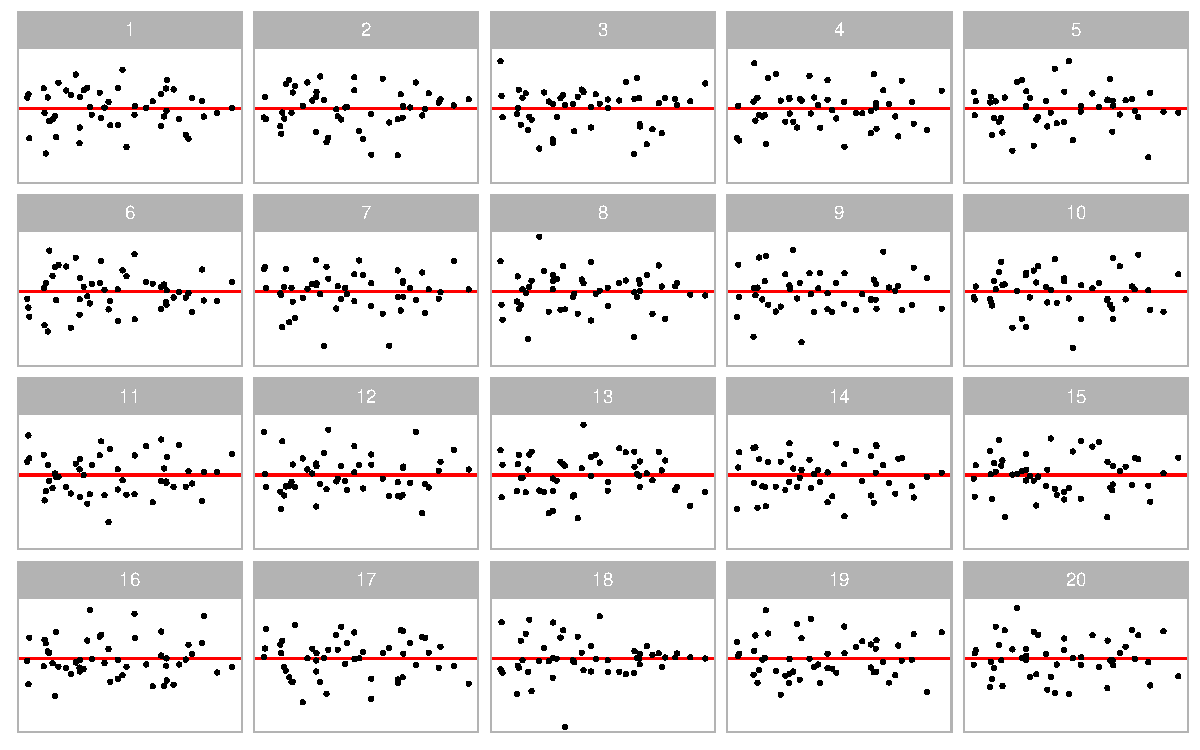
\includegraphics[width=1\linewidth]{paper_comparison_files/figure-latex/easy-heter-example2-1} 

}

\caption{Lineup heter-536 with $log_e(E) = 4.13$ produced by the heteroskedasticity model used in experiment II. It is rejected by the visual test but not by the  Breusch-Pagan test. The data plot at panel 18 exhibits a vague heteroskedasticity pattern, but it contains a distinct outlier which makes it attractive to subjects.}\label{fig:easy-heter-example2}
\end{figure}

\hypertarget{moderate-lineup}{%
\subsubsection{Moderate lineup}\label{moderate-lineup}}

With the increase of the difficulty level, the sensitivity of
conventional tests enlarge the difference in rejection rates. For
moderate lineup produced by the non-linearity model, 8\% and 28\% are
rejected and accepted by both tests respectively. We can observe a
decline in agreement rate to 36\%. A large proportion of lineups are
accepted by the visual test and rejected by the conventional test, which
is around 63\%. The remaining 1\% are rejected by conventional tests
only, which suffer the same issue caused by the RESET test as mentioned
earlier.

For those produced by the heteroskedasticy model, the corresponding
numbers are 23\%, 31\%, 54\%, 45\% and 1\%. There is only one lineup
rejected by the visual test but accepted by the conventional test. It
does not show any heteroskedasticity patterns, but contains a few
outliers at the bottom of the data plot as illustrated in panel 14 of
Figure \ref{fig:moderate-heter-example1}. Two out of five subjects
correctly identify this lineup yielding a \(p\)-value equal to
\(0.044\). We consider this instance is rejected by chance. If a
different set of null plots are used, the data plot may not be
identified.

\begin{figure}

{\centering 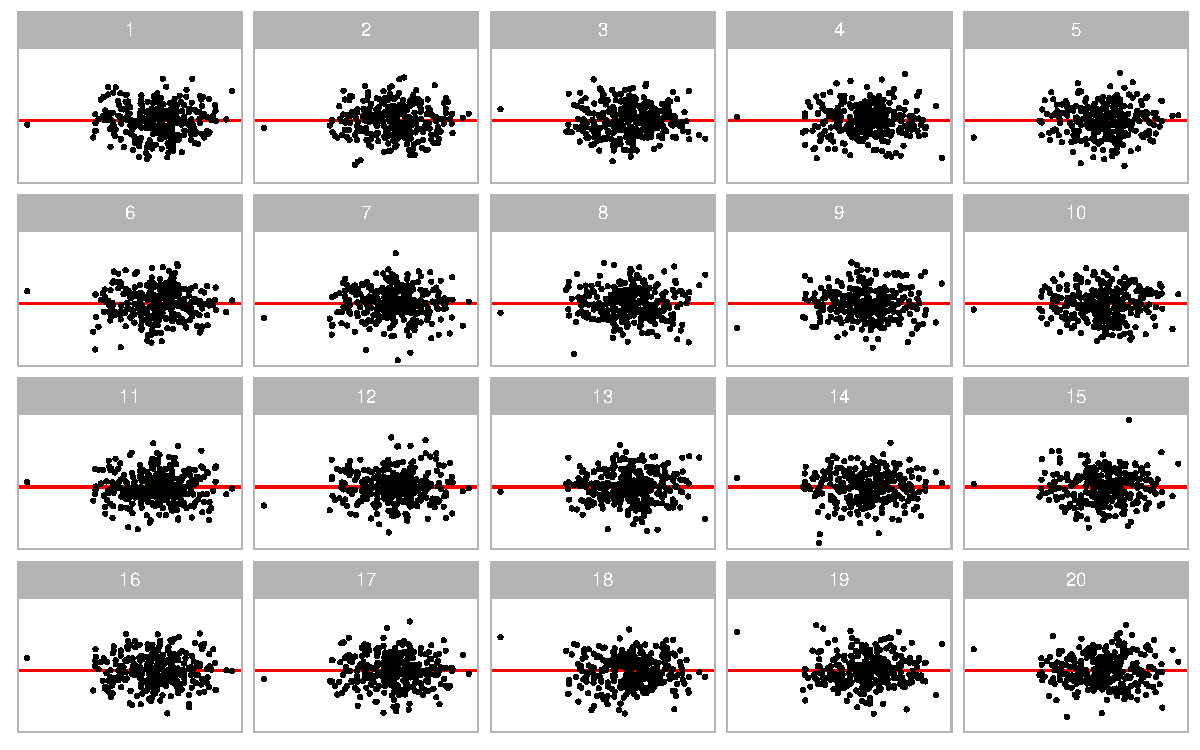
\includegraphics[width=1\linewidth]{paper_comparison_files/figure-latex/moderate-heter-example1-1} 

}

\caption{Lineup heter-219 with $log_e(E) = 1.61$ produced by the heteroskedasticity model used in experiment II. It is rejected by the visual test but not by the  Breusch-Pagan test. Though the data plot at panel 14 shows no heteroskedasticity patterns, it contains a few outliers at the bottom of the panel.}\label{fig:moderate-heter-example1}
\end{figure}

\hypertarget{difficult-lineup}{%
\subsubsection{Difficult lineup}\label{difficult-lineup}}

Visual test is insensitive to lineups with small effect. When it comes
to difficult level, none of the lineups produced by the non-linearity
model are rejected by the visual test. There are 73\% of lineups
accepted by both tests, and 26\% rejected by the conventional test. The
agreement rate rise up to 73\%.

For lineups produced by the heteroskedasticity model, 3\% are rejected
by both tests, and 71\% are accepted by both tests. There are 24\% of
lineups rejected by the conventional test only. Besides, only two
lineups, which is 2\% of all the difficult lineups, are rejected by the
visual test only.

As shown in \ref{fig:difficult-heter-example1} and
\ref{fig:difficult-heter-example2}, residual plots of both lineups are
constructed with \(X_{raw} \sim lognormal(0, 0.6^2)/3\). Though the
designed patterns are ``Left-triangle'' and ``Butterfly'' shape, both of
them are invisible due to the small effect. The visual effect are
dominated by the skewed distribution. Further, no distinguishable visual
patterns, such as outliers, are detectable from the data plot of these
two lineups, which are panel 5 and panel 15. The data plots in these two
lineups are not the most different plot from our point of view either.
However, three out of five and two out of five subjects correctly
identify the data plot for these two lineups respectively. But the
reasons for selecting the plot provided by the subjects are mixed and
inconsistent. Hence, with the current data, we can not explain why
subjects can correctly identify the data plot of these two lineups.
Collecting more data in future study may help to answer this question.

\begin{figure}

{\centering 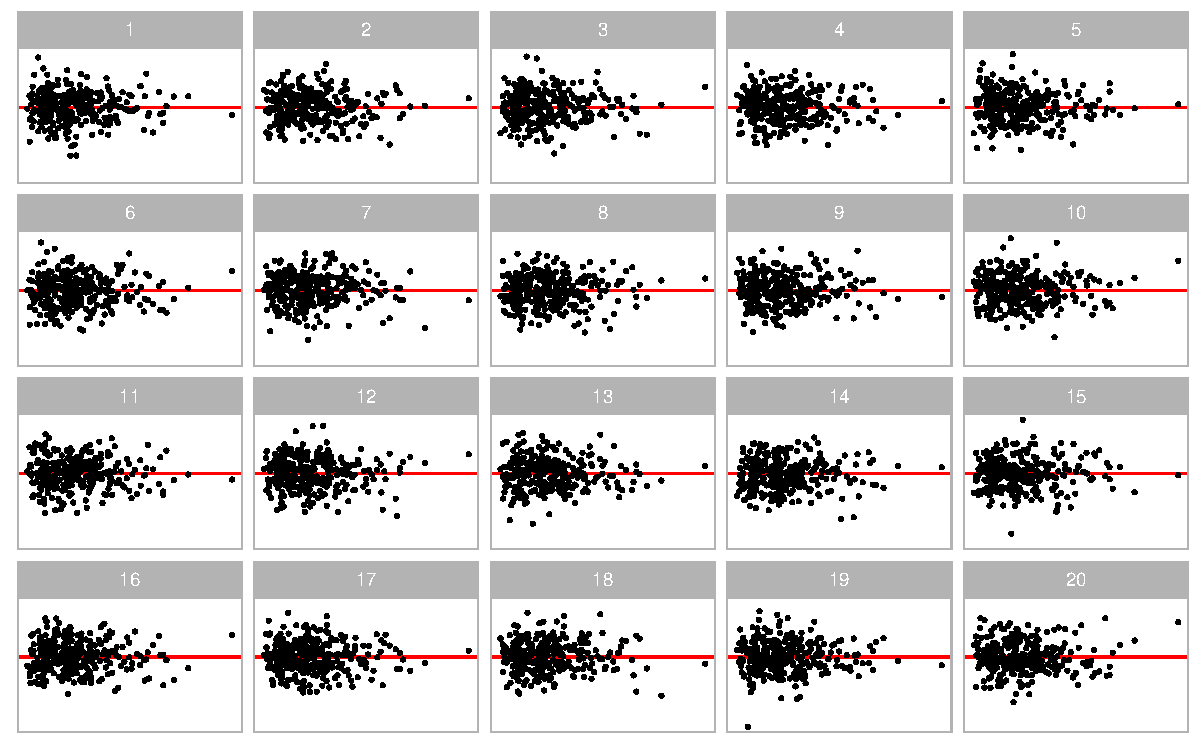
\includegraphics[width=1\linewidth]{paper_comparison_files/figure-latex/difficult-heter-example1-1} 

}

\caption{Lineup heter-224 with $log_e(E) = 1.32$ produced by the heteroskedasticity model used in experiment II. It is rejected by the visual test but not by the  Breusch-Pagan test. Although two out of five subjects correctly identify the data plot at panel 5, it does not exhibit any visually distinguishable pattern.}\label{fig:difficult-heter-example1}
\end{figure}

\begin{figure}

{\centering 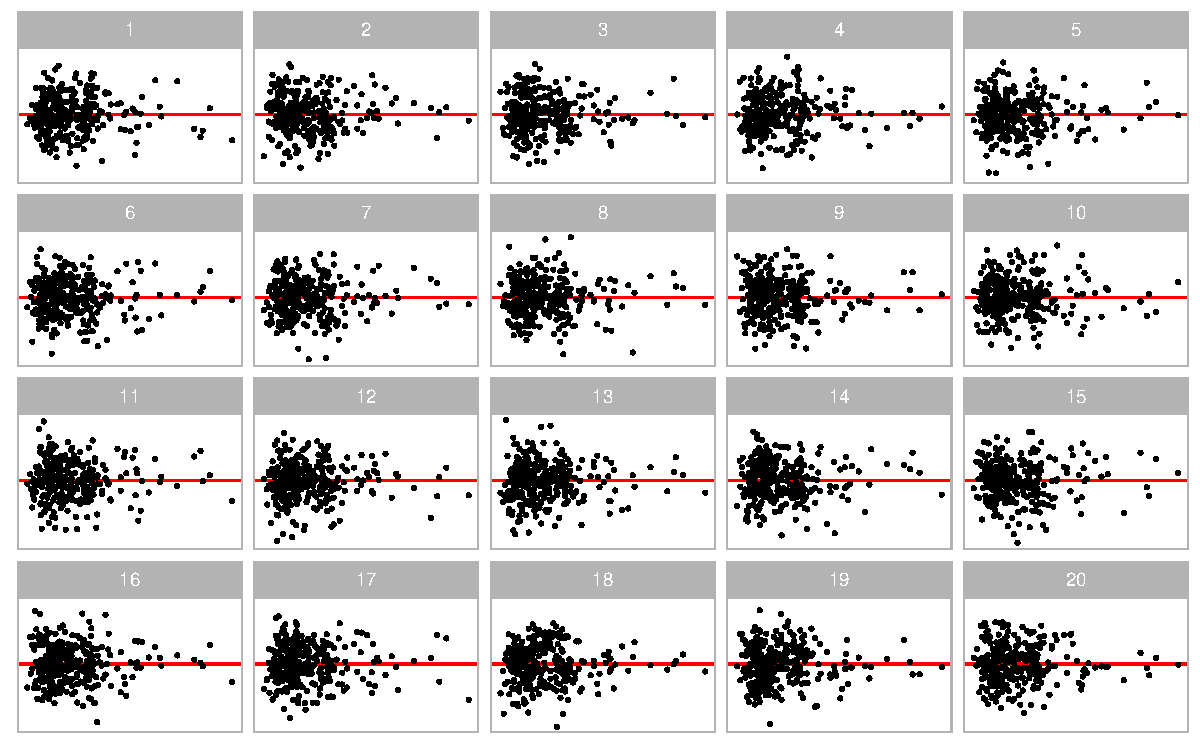
\includegraphics[width=1\linewidth]{paper_comparison_files/figure-latex/difficult-heter-example2-1} 

}

\caption{Lineup heter-415 with $log_e(E) = -0.31$ produced by the heteroskedasticity model used in experiment II. It is rejected by the visual test but not by the  Breusch-Pagan test. Panel 15 is the data plot but it does not exhibit any visually distinguishable pattern.}\label{fig:difficult-heter-example2}
\end{figure}

\begin{figure}

{\centering 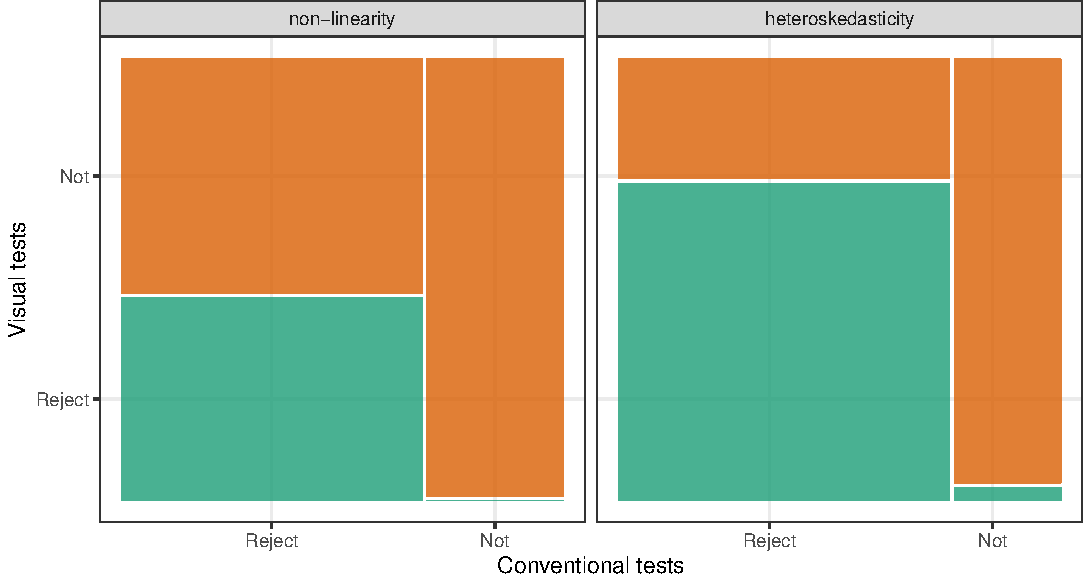
\includegraphics[width=1\linewidth]{paper_comparison_files/figure-latex/p-value-comparison-1} 

}

\caption{Rejection rate of visual test compared to conventional test on lineups produced by heteroskedasticity and non-linearity model at different levels of difficulty. Based on the rejection decision made by the visual test and the conventional test, the mosaic plot shows the proportion of lineups in each category.}\label{fig:p-value-comparison}
\end{figure}

\hypertarget{effect-of-the-distribution-of-the-regressor}{%
\subsection{Effect of the distribution of the
regressor}\label{effect-of-the-distribution-of-the-regressor}}

\begin{center}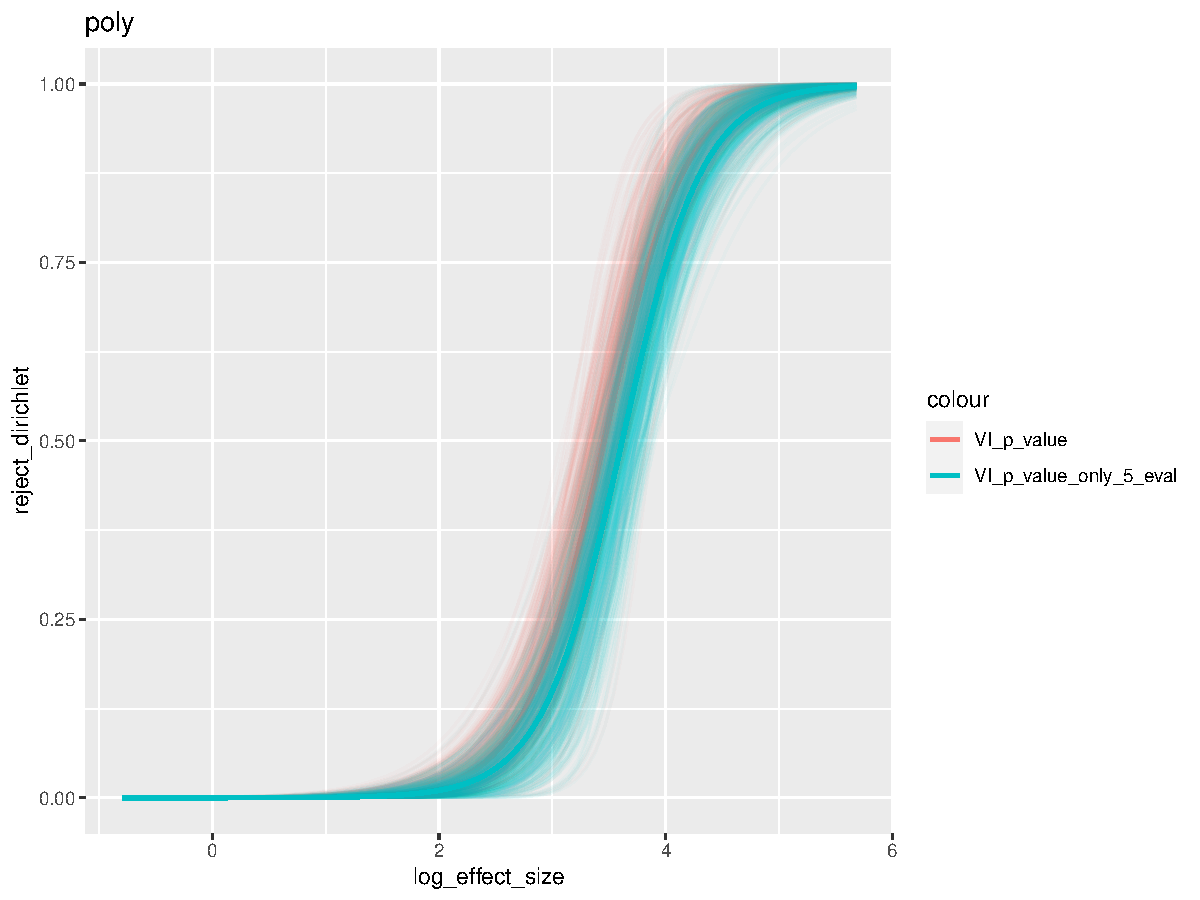
\includegraphics[width=1\linewidth]{paper_comparison_files/figure-latex/unnamed-chunk-14-1} \end{center}

\begin{center}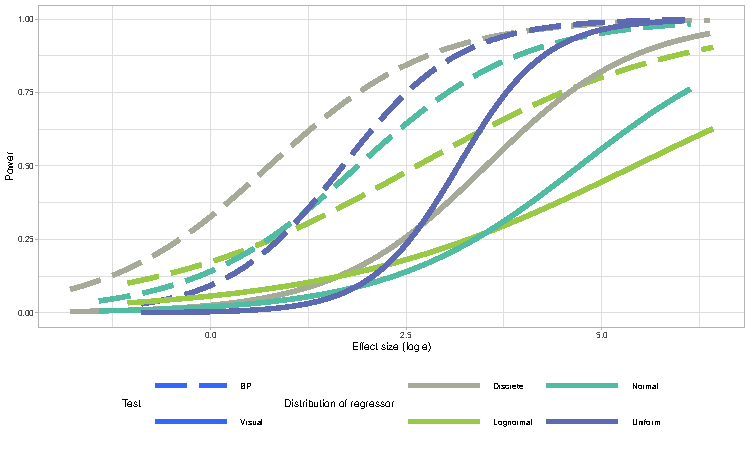
\includegraphics[width=1\linewidth]{paper_comparison_files/figure-latex/unnamed-chunk-15-1} \end{center}

(change of x\_dist -\textgreater{} power)

\hypertarget{appendix}{%
\section{Appendix}\label{appendix}}

\hypertarget{effect-derivation}{%
\subsection{Effect derivation}\label{effect-derivation}}

\hypertarget{p-value-scatter-plot}{%
\subsection{\texorpdfstring{\(p\)-value scatter
plot}{p-value scatter plot}}\label{p-value-scatter-plot}}

\hypertarget{a-collection-interesting-lineups-unusual-results}{%
\subsection{A collection interesting lineups (unusual
results)}\label{a-collection-interesting-lineups-unusual-results}}

why unusual? what is the possible explanations?

\hypertarget{targe-journal}{%
\section{targe journal}\label{targe-journal}}

JRSSB: Journal of the Royal Statistical Society Series B (Statistical
Methodology) Deadline: Jan 1, Apr 1

Reading: style of writing, author guideline
(\url{https://rss.onlinelibrary.wiley.com/hub/journal/14679868/author-guidelines})

JCGS JDSS

\bibliographystyle{tfcad}
\bibliography{paper.bib}





\end{document}
